%%% %%%%%%%%%%%%%%%%%%%%%%%%%%%%%%%% %%%
%%% Main Chapter 4 : Implementation  %%%
%%% %%%%%%%%%%%%%%%%%%%%%%%%%%%%%%%% %%%
\chapter{Setup}
\label{chap:setup}

	In diesem Kapitel wird beschrieben, wie ausgewählte historische Betriebssysteme im Rahem dieser Arbeit wieder lauffähig gemacht wurden. Als Hypervisor kam, sofern nicht anderweitig vermerkt, VMWare Fusion Professional Version 6.0.2 auf Mac OS 10.9.2 zum Einsatz. 
	Die VMs werden zusammen mit dieser Arbeit eingereicht.

%%%%%%%%%%%%%%%%%%%%%%%%%%%%%%%%%%%%%%%%%%%%%%%%%%%%%%%%%%%%%%%%%%%%%%%%%%%%%%%%%%%%%%%%%%%%%%%%%%%%%%%%%
\section{PC DOS 1.10}
%%%%%%%%%%%%%%%%%%%%%%%%%%%%%%%%%%%%%%%%%%%%%%%%%%%%%%%%%%%%%%%%%%%%%%%%%%%%%%%%%%%%%%%%%%%%%%%%%%%%%%%%%

	MS DOS 1.0 stellt das erste Betriebssystem von Microsoft für die 8086-CPU dar. Es entstand durch eine Portierung von Tim Patersons QDOS auf den IBM PC und wurde mit diesem unter dem Namen IBM PC DOS vertrieben. \cite{WinHistory}
	Beim hier verwendeten PC DOS 1.10 handelt es sich um eine fehlerbereinigte, im Juli '82 veröffentlichte Version, die technisch MS DOS 1.25 entspricht. 
	Dieses Betriebssystem stelltgrößtenteils einen Nachbau von CP/M dar und war, außer durch das Vorhandensein des Dateisystems \gls{FAT}, wenig innovativ.
	Da es jedoch die Grundlage für den Erfolg von Microsoft und somit für alle späteren Betriebssysteme bildet, wird es in dieser Arbeit behandelt.

	DOS unterstützt in der Version 1 noch keine Festplatten und kann lediglich 5,25" Disketten bis 160 KB adressieren. \cite{WinHistory}
	Unter anderem aufgrund dieser Einschränkungen kann dieses Betriebssystem nicht mit zeitgemäßen Hypervisoren ausgeführt werden, statt dessen muss ein vollwertiger CPU- bzw. PC-Emulator wie Bochs oder QEMU verwendet werden. 

	Im "`Endangered Software Archive"', welches unter der URL \url{http://www.mirrors.org/archived_software/www.techknight.com/esa/default.htm} verfügbar ist, befindet sich eine mit dem "`Disk Image Archiver"' erstellte Kopie der originalen PC DOS 1.10 Startdiskette. 
	Mit einem Hex-Editor lässt sich aus dem proprietären .dim-Format eine Datei mit dem Inhalt der Diskette erstellen und das Betriebssystem in Bochs booten.
	Dieser Prozess ist in \cite{PCMinistry} beschrieben:

	Der Bootsektor der Diskette entspricht noch nicht den gängingen Industriestandards.
	So fehlt der BIOS Parameter Block, der bei allen FAT (ab DOS 2.0) und NTFS Dateisystemen den Aufbau des Datenträgersbeschreibt und Informationen über das Dateisystem enthält. Im vorliegenden Image ist dieser Bereich (ab Offsett 07h) freigelassen.
	Modernere Betriebssysteme können die Diskette daher nicht lesen und geben aus, der Datenträger sei nicht korrekt formattiert. 
	Zudem wird die "`Boot Sektor Signatur"' am Ende des ersten Sektors (55h bei Offsett 1FEh und AAh bei Offsett 1FFh), welche ein Medium als bootbar markiert, vom BIOS bei Start noch nicht überprüft. \cite{IBMTechRef} Daher fehlt auch diese auf der Diskette und in dem Image sind am Ende des Bootsektors lediglich Nullen zu finden.
	Daher verweigert der Emulator den Bootvorgang.
	Ändert man mit einem Hex-Editor die Datei und schreibt 55AA an das Ende des Bootsektors, übergibt das BIOS die Kontrolle mittels JMP-Befehl an den in dem Image liegenden Code. Leider stürzt das System dann beim Bootvorgang ab.

	\begin{figure}[h]
		\begin{center}
			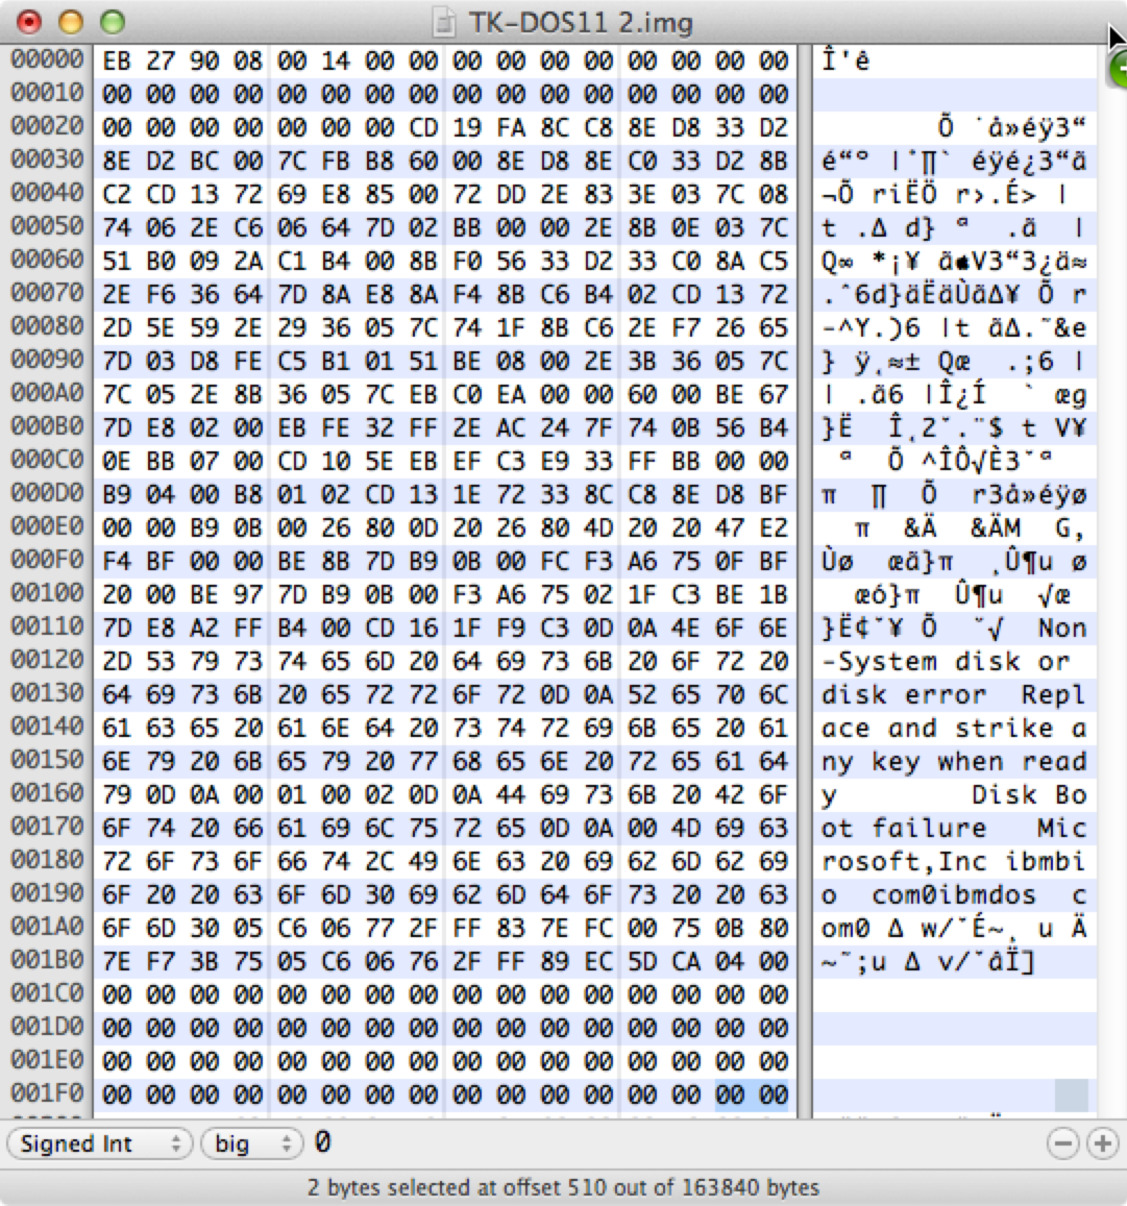
\includegraphics[width=0.7\textwidth]{img/DOS110hex}
			\caption{Ansicht des PC DOS 1.10 Bootsektors im Hex-Editor}
			\label{fig:screenshot-hexeditor110}
		\end{center}
	\end{figure}

	Glücklicherweise bietet Bochs bietet jedoch die Möglichkeit, die Überprüfung der Signatur zu deaktivieren und jeglichen Programmcode sofort zu booten, indem man \lstinline{floppy_bootsig_check: disabled=1} in das config file schreibt.
	Ein funktionierendes config File wird unter dem Namen $bochs.txt$ mit dieser Arbeit ausgeliefert.
	Hiermit lässt sich ein unverändertes Image von PC DOS 1.10 ausführen.
	Hierzu muss bochs im entsprechenden Verzeichnis gestartet werden, die Option \lstinline{2. Read options from ...} gewählt werden, mittels \lstinline{6. Begin simulation} der Emulator geladen werden und mit dem Befehl $continue$ die CPU gestartet werden.

	\begin{figure}[p]
		\begin{center}
			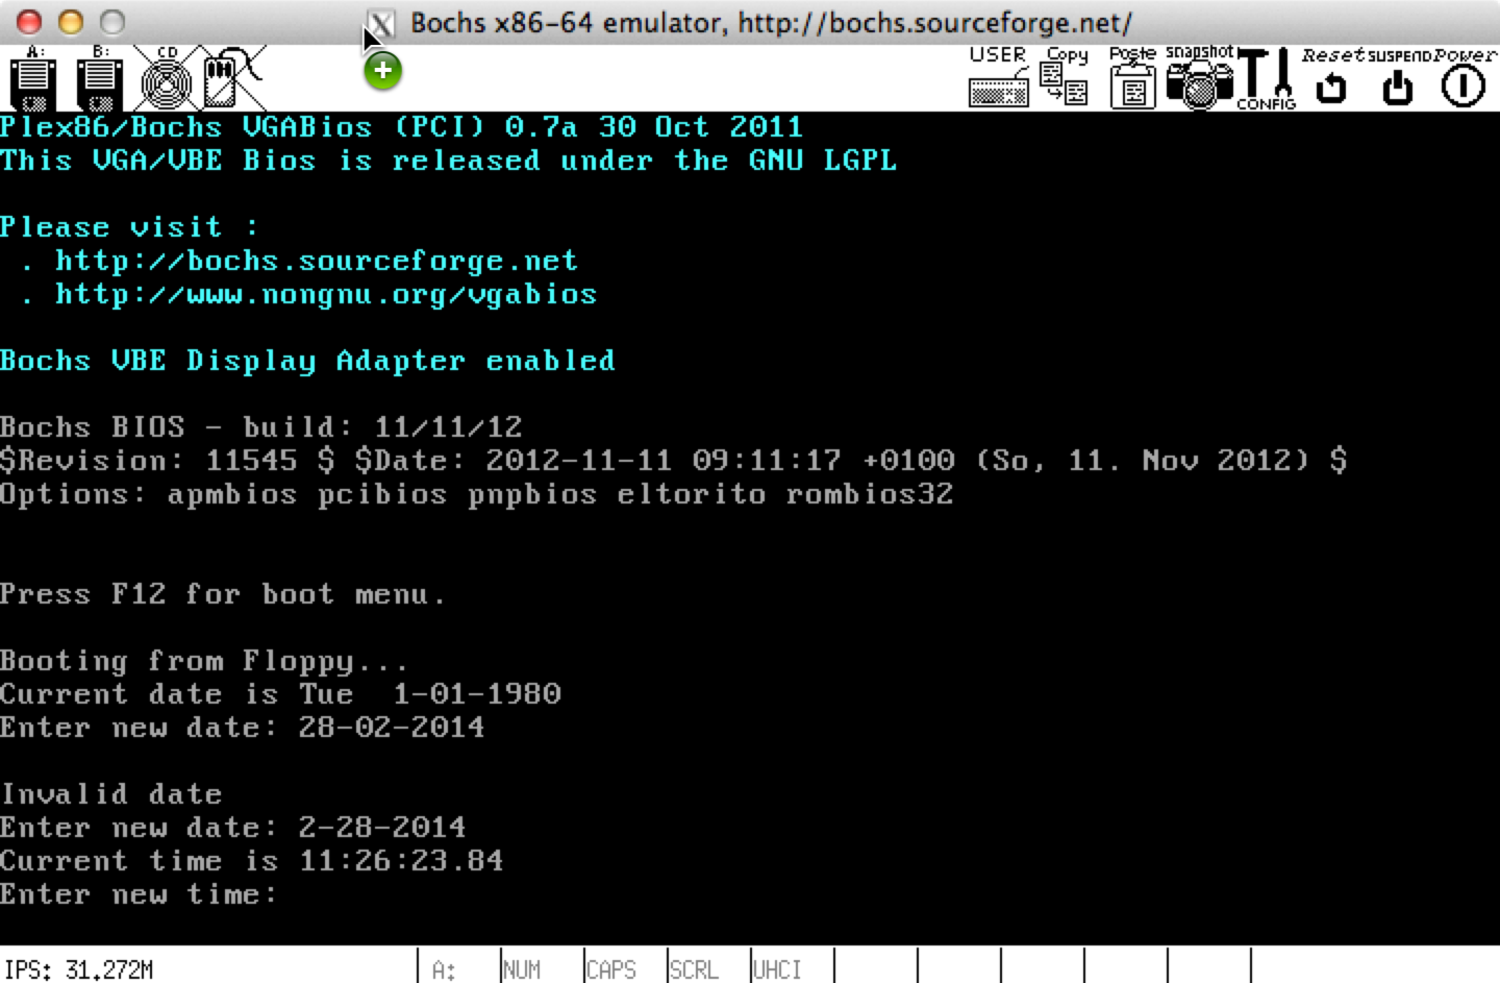
\includegraphics[width=\textwidth]{img/DOS110_1}
			\caption{Bootscreen von DOS 1.10}
			\label{fig:screenshot-dos110boot}
		\end{center}
	\end{figure}

	\begin{figure}[p]
		\begin{center}
			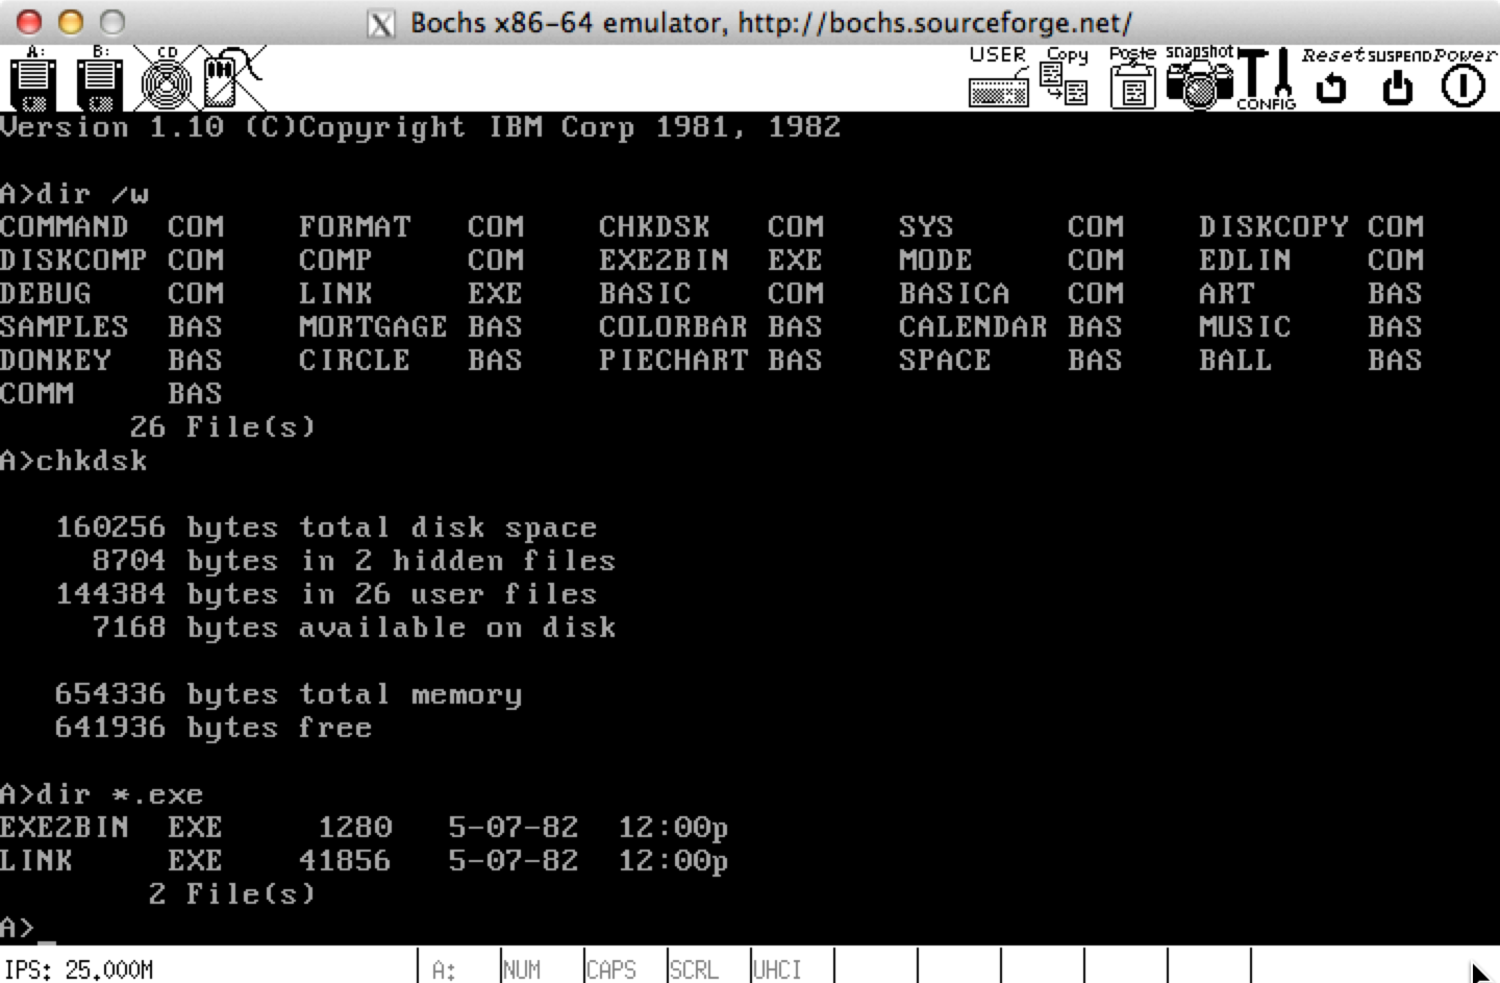
\includegraphics[width=\textwidth]{img/DOS110_2}
			\caption{Kommandos in PC DOS 1.10}
			\label{fig:screenshot-dos110commands}
		\end{center}
	\end{figure}

	Leider sind auch hier bei weitem nicht alle Funktionen des Betriebssystems benutzbar, da MS DOS sämtliche I/O-Operationen über die BIOS-Routinen durchführt.
	Das im originalen IBM PC verwendete BIOS unterscheidet sich jedoch signifikant von der "`BIOS Boot Specification"' vom 11. Januar 1996 und ist daher mit dem verwendeten Plex86/Bochs VGABios nicht kompatibel.

\newpage

%%%%%%%%%%%%%%%%%%%%%%%%%%%%%%%%%%%%%%%%%%%%%%%%%%%%%%%%%%%%%%%%%%%%%%%%%%%%%%%%%%%%%%%%%%%%%%%%%%%%%%%%%
\section{DOS 5.0 \& Windows 2.11}
%%%%%%%%%%%%%%%%%%%%%%%%%%%%%%%%%%%%%%%%%%%%%%%%%%%%%%%%%%%%%%%%%%%%%%%%%%%%%%%%%%%%%%%%%%%%%%%%%%%%%%%%%

	MS DOS 5.0 erschien im im Juni 1991.
	In den 10 Jahren seit der Veröffentlichung von PC-DOS 1.0 hatten sich zahlreiche Veränderungen ergeben. 
	Das Betriebssystem konnte nun auf Festplatten installiert werden, unterstütze 3,5''-Diskettenlaufwerke mit 720 KB, kannte Verzeichnisse in FAT, und konnte mittels Expanded Memory Specificatgion Arbeitsspeicher von mehr als 1 MB adressieren. 

	Windows 2.11 stellte einen Meilenstein dar, da es das erste Microsoft-Betriebssystem war das den protected mode des 386er Prozessors benutzte. Zudem bot es VGA-Unterstützung und neben kooperativem Multitasking auch die Möglichkeit, Fenster überlappen zu lassen.

	\begin{figure}[h]
		\begin{center}
			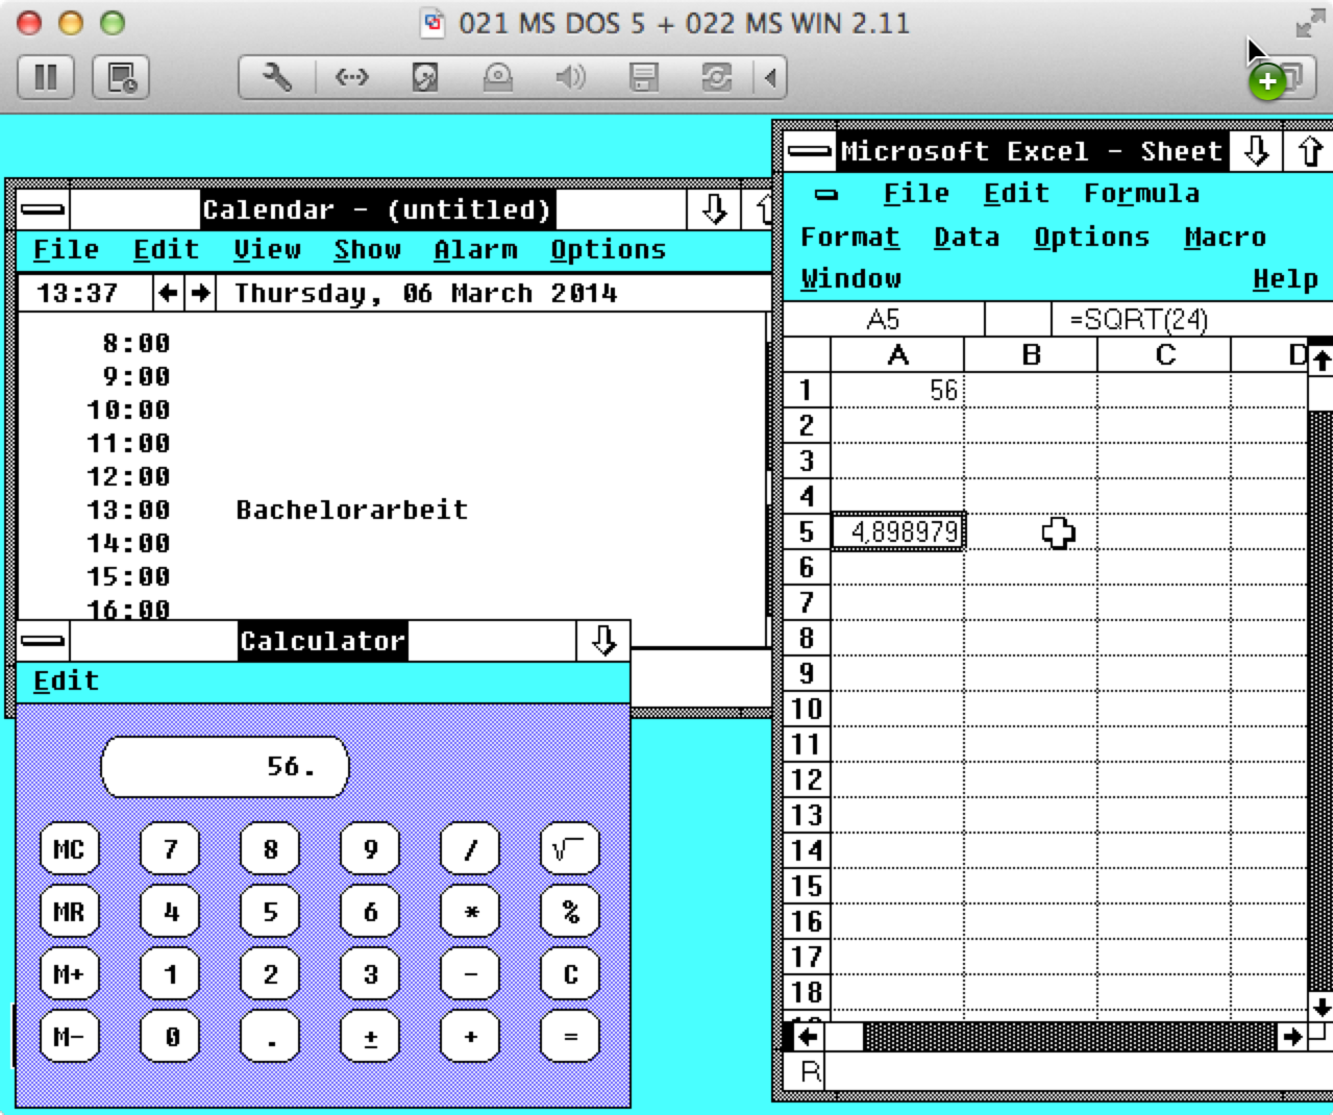
\includegraphics[width=\textwidth]{img/WIN211_2}
			\caption{Windows 2.11 mit Excel und einigen Standardprogrammen}
			\label{fig:screenshot-win211excel}
		\end{center}
	\end{figure}

	Im Rahmen dieser Arbeit wurden DOS 5.0 und Windows 2.11 auf 3,5''-Disketten gebraucht erworben und zudem ein USB-Floppylaufwerk bezogen.
	Leider gelang es nicht, diese originalen Disketten mit je 720 KB ("`Double Density"') auszulesen, da alle heutigen Betriebssysteme nur noch das Ansprechen von 1,44 MB-Datenträgern ("`High Density"') beherrschen.
	Versuche, den Inhalt der Disketten auszulesen schlagen daher mit der Meldung $I/O-Error$ fehl.
	Mit einem zufällig bei Autor noch vorhandenen Rechner mit Windows 95 war es ebenfalls nicht möglich die Daten auszulesen, da das integrierte Diskettenlaufwerk durch Alterung nicht mehr funktionierte.

	Images von beiden Systemen sind jedoch bei WinWorld\footnote{\url{http://wdl2.winworldpc.com/Abandonware\%20Operating\%20Systems/PC/DOS/Microsoft/}}, einem selbsternannten Online-Museum für Software verfügbar.
	Diese Images können in einer virtuellen Maschine als Diskettenlaufwerk gebootet werden, wenn als Betriebssystem MS-DOS konfiguriert und eine IDE-Festplatte mit weniger als 32 MB angelegt wird.
	Die Installation und der Betrieb von MS-DOS funktoinieren problemlos, allerdings kann nur RAM bis 1 MB adressiert werden.
	Dies gestaltet den Betrieb von Windows 2.11 kompliziert, aber nicht unmöglich.
	Bei der Installation muss explizit ausgewählt werden, Windows ohne extended memory installieren zu wollen, dann gelingt der Start.

	Einer der Hauptgründe für den Betrieb von Windows in der Version 2 war die Notwendigkeit, Excel ausführen zu müssen.
	Excel bringt eine eingeschränkte Windows-Runtime mit, damit es auch ohne eine Lizenz für Windows auf DOS-Rechnern ausgeführt werden kann.
	Es läuft jedoch besser unter einer Vollversion von Windows. 
	Zudem lassen sich damit bspw. Kalendereinträge übernehmen und Daten aus anderen Prozessen  kopieren.
	Aufgrund des historischen Kontexts, wird mit dieser VM eine Installation von Excel 2.1d mitgeliefert.

	Bei der Installation von Excel fällt auf, dass es in den gleichen Ordner wie Windows installiert werden muss (i.d.R. $C:\backslash{}Windows$). Zudem bringt es ein Programm namens $MemSet$ mit, welches den erweiterten Arbeitsspeicher konfiguriert und neue RAM-Treiber installiert. Mit diesem gelingt auch die Benutzung von RAM jenenseits der 1 MB.



	\begin{figure}[h]
		\begin{center}
			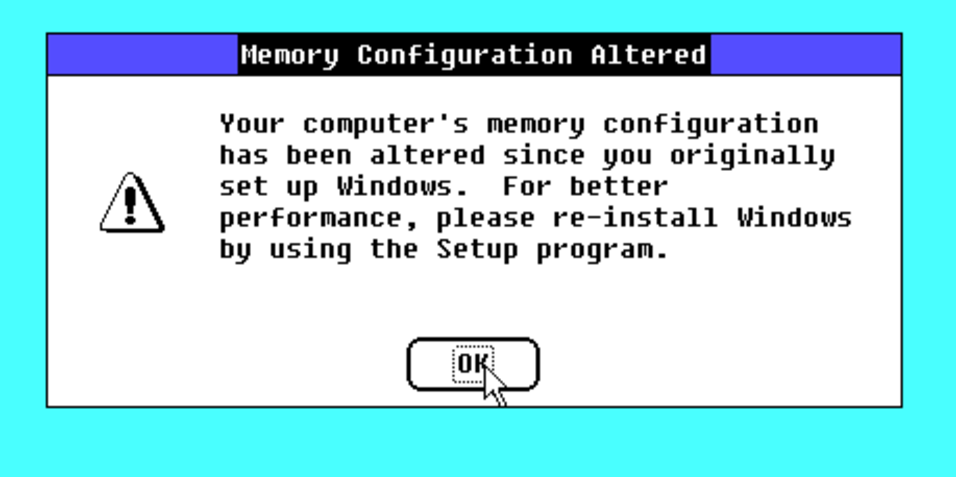
\includegraphics[width=0.7\textwidth]{img/WIN211_1}
			\caption{Warnung beim Start von Windows 2.11 nach der Installation von Excel}
			\label{fig:screenshot-win211error}
		\end{center}
	\end{figure}

\newpage

%%%%%%%%%%%%%%%%%%%%%%%%%%%%%%%%%%%%%%%%%%%%%%%%%%%%%%%%%%%%%%%%%%%%%%%%%%%%%%%%%%%%%%%%%%%%%%%%%%%%%%%%%
\section{DOS 6.0 \& Windows 3.11}
%%%%%%%%%%%%%%%%%%%%%%%%%%%%%%%%%%%%%%%%%%%%%%%%%%%%%%%%%%%%%%%%%%%%%%%%%%%%%%%%%%%%%%%%%%%%%%%%%%%%%%%%%
	Windows der dritten Generation war die erste auch bei Privatanwendern beliebte und kommerziell erfolgreiche Version des graphischen Betriebssystems von Microsoft.
	Zusätzlich wurde bei Version 3.11 Netzwerkfunktionalität eingeführt.

	Aus der gleichen Zeit stammt MS DOS der 6. Generation \cite{WinHistory}, eine stabile und zuverlässige Version, die unter anderem die Dateisystemkomprimierung DoubleSpace mitbringt.

	Beide Systeme wurden in einem Set aus mehreren 1,44 MB Disketten ausgeliefert und fanden sich noch im Keller der Eltern des Autors.
	Diese konnten problemlos mit einem USB-Floppylaufwerk und dem Befehl $dd$ in eine Image-Datei kopiert werden.
	Trotz ihres Alters hatte keine der Disketten defekte Sektoren.

		\begin{figure}[h]
		\begin{center}
			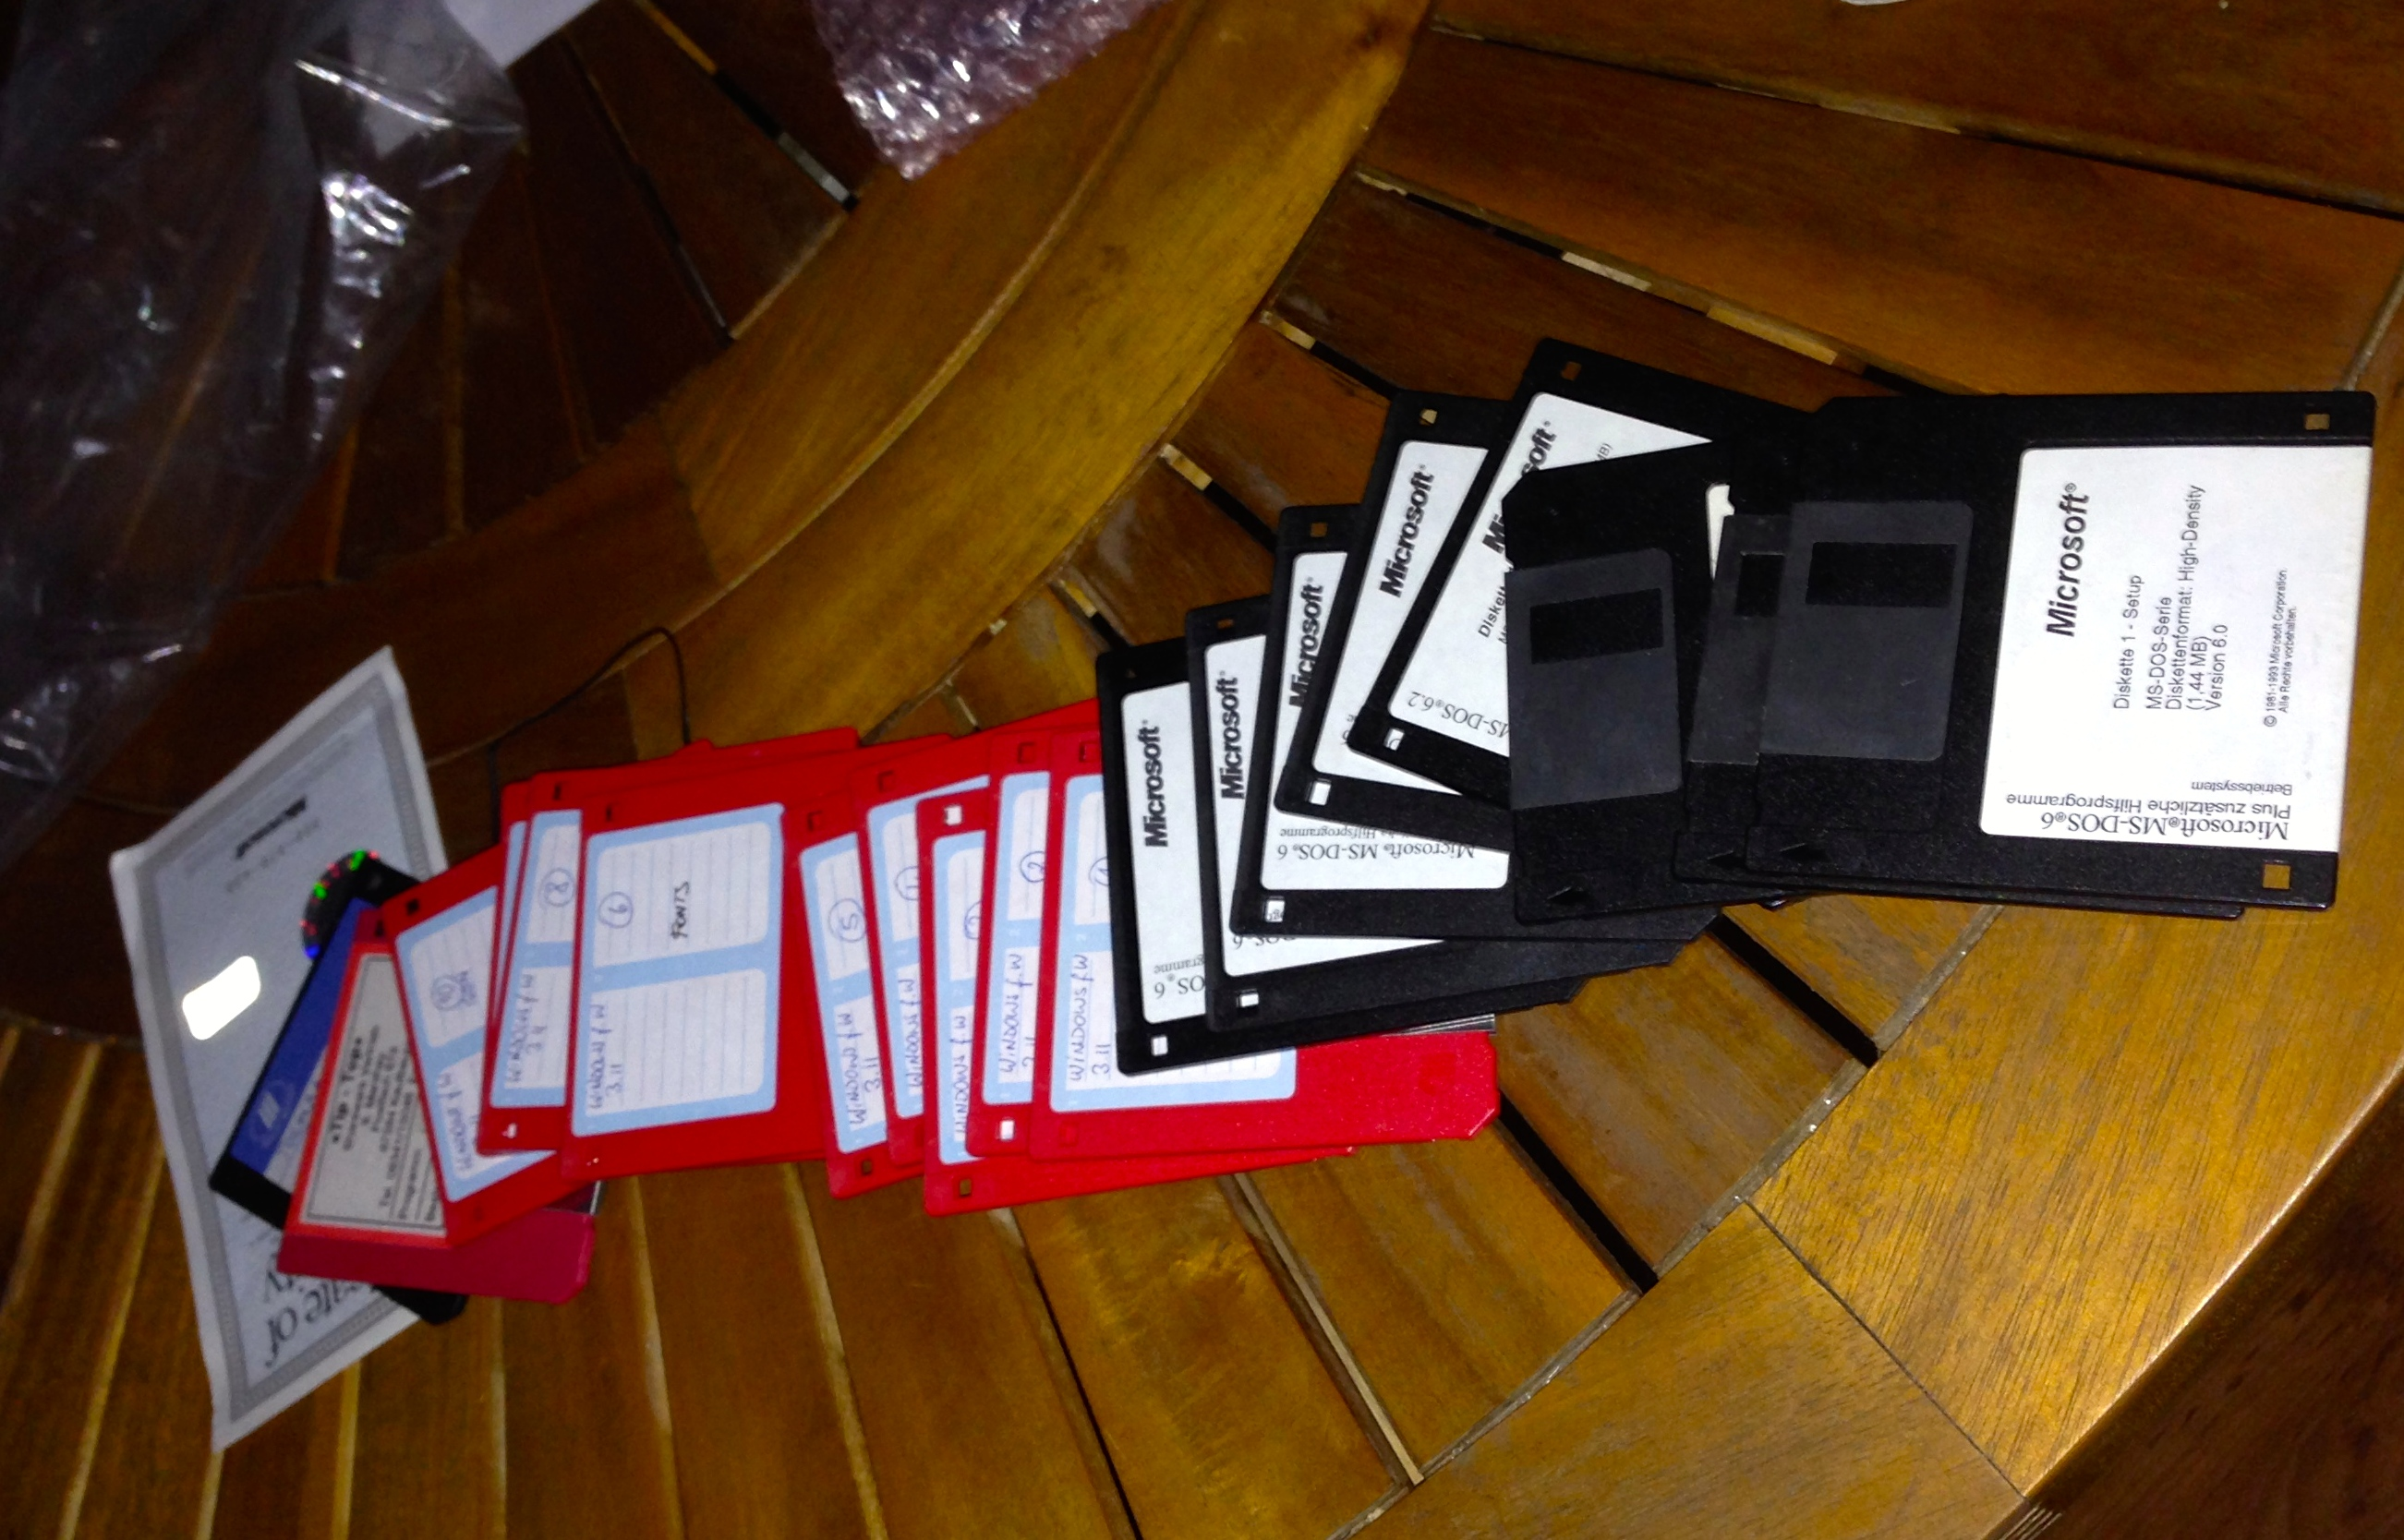
\includegraphics[width=0.8\textwidth]{img/win311disks.jpg}
			\caption{Windows 3.11 und MS DOS 6.22 auf Disketten}
			\label{fig:screenshot-win311disks}
		\end{center}
	\end{figure}

	Stellt mal VMWare in den Kompatibilitätseinstellungen auf Version 8 des Hypervisors um, kennt es einen Modus für Windows 3.11, indem sich das Betriebssystem problemlos von den Diskettenimages installieren lässt. Leider gibt es keine VMWare Guest Additions für dieses Betriebssystem und somit funktionieren nach Installation weder Sound, Netzwerk noch CDROM\footnote{Die in diesem Kapitel installierten Treiber wurden alle von \cite{VMDriver} geladen}.

	Da sowohl MS DOS als auch Windows vor Version 95 im Leerlauf busy waiting statt dem $HLT$-Befehl verwenden, ist die CPU der virtuellen Maschine zudem immer vollständig ausgelastet.
	Dies ist besonders auf einem zentralen Cloud-System, bei dem viele virtuelle Maschinen parallel ausgeführt werden sollen sehr störend, da jede VM die ihr zur Verfügung stehenden Ressourcen somit voll belegt, auch wenn sie nicht benutzt werden.
	Eine Lösung findet sich auf \cite{VMDriver} mit dem Programm "`CPUidle for DOS"' von Marton Balog.
	Bei diesem handelt es sich um eine TSR, die das busy waiting von MS DOS überschreibt, statt dessen die CPU in dieser Zeit anhält und durch Interrupts wieder aufweckt.
	Gleiches bewirkt unter Windows 3.11 der Treiber "`WQGHLT"' aus der selben Quelle.

	\begin{figure}[h]
		\begin{center}
			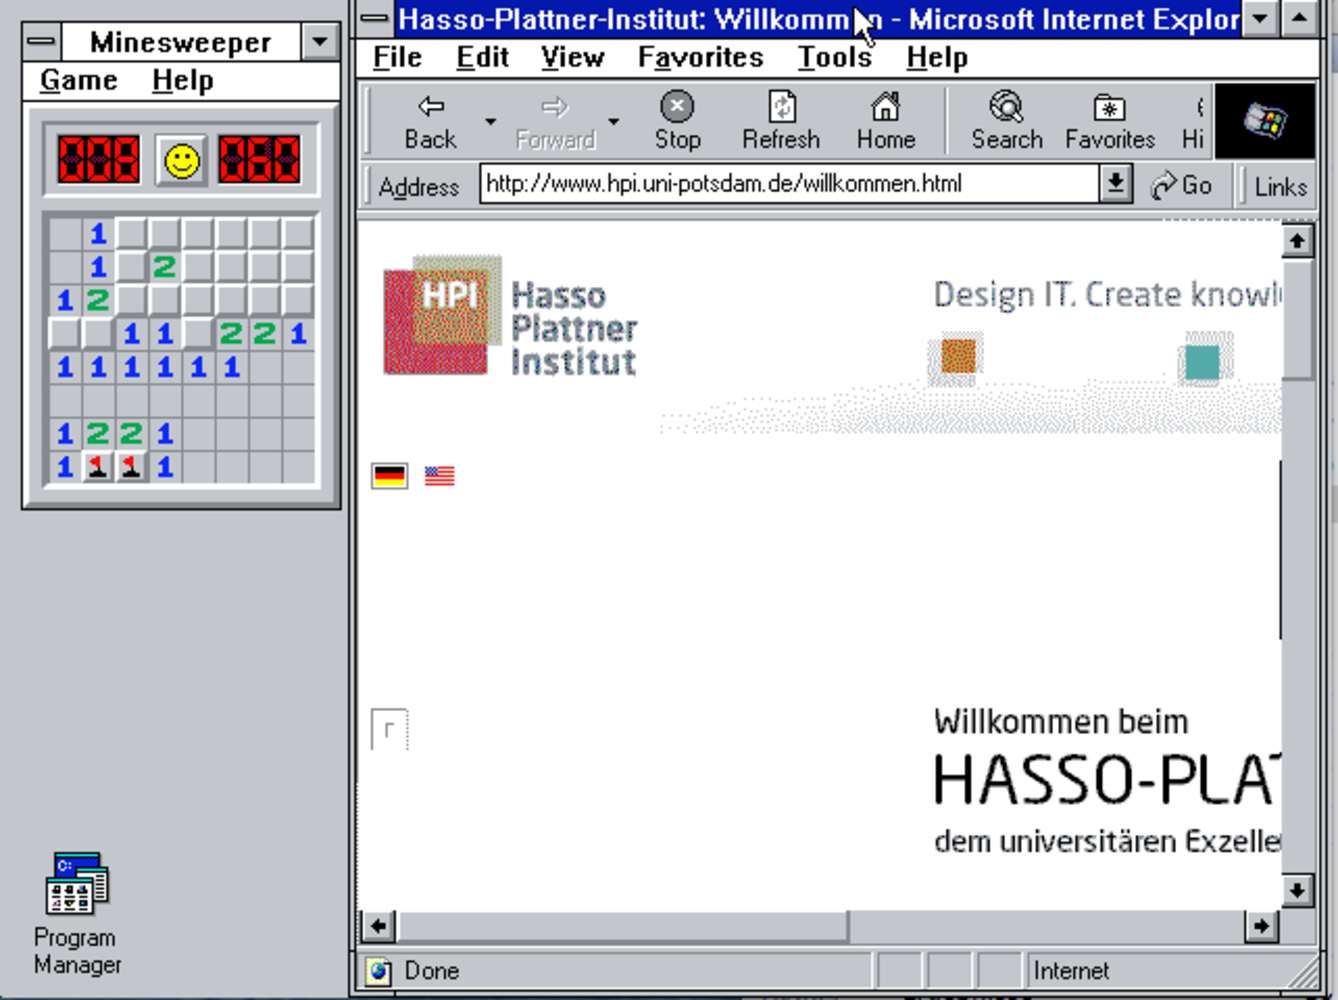
\includegraphics[width=\textwidth]{img/win311screen}
			\caption{Windows 3.11 mit Minesweeper und Internet Explorer 5.0}
			\label{fig:screenshot-win311apps}
		\end{center}
	\end{figure}

	Die Netzwerkfuntkionalität kann aktiviert werden, indem der Treiber für die "`Advanced Micro Devices PCNET Family"' nachinstalliert wird.
	Zudem muss explizit der TCP/IP-Protokolltreiber installiert werden, da Windows 3.11 standardmäßig nur die veralteteten Protokollen IPX/SPX und NetBEUI unterstützt.

	Leider nicht mehr aktivieren lässt sich die Unterstützung für Audioausgabe, da VMWare die Karte SoundBlaster16 nur bis zur Version 6 emuliert.
	Neuere Hypervisoren emulieren leistungsfährigere Soundkarten, für die es aber keine Treiber mehr für Windows 3.11 gibt.


	Bei WinWorld finden sich außerdem auf diesem Betriebssystem lauffähige Versionen von Internet Explorer und Netscape Navigator.
	Letzterer stürzt aufgrund eines Bugs jedoch im Hypervisor und auf neueren CPUs als Pentium ab, dabei bringt er Windows komplett zum Absturz und ist ein gutes Beispiel für den fehlenden Speicherschutz.

	Der Internet Explorer lässt sich hingegen in Version 5.0 installieren und ausführen. 
	Hiermit lässt sich ansatzweise im Internet surfen, jedoch werden nahezu alle Webseiten werden fehlerhaft dargestellt, da noch kein CSS der Version 2 unterstützt wird und außerdem nur Seiten bis zu einer Größe von 1 MB verarbeitet werden können. \\



\newpage

%%%%%%%%%%%%%%%%%%%%%%%%%%%%%%%%%%%%%%%%%%%%%%%%%%%%%%%%%%%%%%%%%%%%%%%%%%%%%%%%%%%%%%%%%%%%%%%%%%%%%%%%%
\section{Windows NT 3.51}
%%%%%%%%%%%%%%%%%%%%%%%%%%%%%%%%%%%%%%%%%%%%%%%%%%%%%%%%%%%%%%%%%%%%%%%%%%%%%%%%%%%%%%%%%%%%%%%%%%%%%%%%%

	Als besonders schwierig gestaltete sich die Verwendung von Windows NT 3.51. 
VM Version manuell runterdrehen, ziemlicher mist
schlecht unterstützt

%%%%%%%%%%%%%%%%%%%%%%%%%%%%%%%%%%%%%%%%%%%%%%%%%%%%%%%%%%%%%%%%%%%%%%%%%%%%%%%%%%%%%%%%%%%%%%%%%%%%%%%%%
\section{Windows NT 4.0 SP 6}
%%%%%%%%%%%%%%%%%%%%%%%%%%%%%%%%%%%%%%%%%%%%%%%%%%%%%%%%%%%%%%%%%%%%%%%%%%%%%%%%%%%%%%%%%%%%%%%%%%%%%%%%%

	Windows NT 4 wird von VMWare unterstützt. 
	Hierbei muss bei der Installation "`Windows NT"' als Betriebssystemtyp gewählt und eine virtuelle SCSI-Festplatte angelegt werden. 
	
	Nach Installation des Service Packs 6a lässt sich der Internet Explorer 6 installieren.
	Damit ist Netzwerkzugriff möglich. 
	Von Microsoft wird ebenfalls ein Post-SP6a Hotfixpaket angeboten \footnote{http://support.microsoft.com/kb/299444/de}, das ebenfalls installiert werden muss, damit die die VMWare Guest Additions funktionieren.

	Nach der Installation der Guest Additions läuft das System stabil und zuverlässig. 

	Um die Updates durchzuführen, wurden die notwendigen Dateien zunächst auf dem Hostsystem heruntergeladen und auf ein ISO-Image kopiert. Dies wurde in VMWares virtuelles CD-Laufwerk geladen und von dort die Installation durchgeführt.

%%%%%%%%%%%%%%%%%%%%%%%%%%%%%%%%%%%%%%%%%%%%%%%%%%%%%%%%%%%%%%%%%%%%%%%%%%%%%%%%%%%%%%%%%%%%%%%%%%%%%%%%%
\section{Windows 2000 Professional}
%%%%%%%%%%%%%%%%%%%%%%%%%%%%%%%%%%%%%%%%%%%%%%%%%%%%%%%%%%%%%%%%%%%%%%%%%%%%%%%%%%%%%%%%%%%%%%%%%%%%%%%%%

Die mitgeliegerte Windows 2000 VM wurde mit einem Datenträger von Maniac, dem Softwareportal für HPI-Studenten, installiert.

Windows 2000 wird von VMware vollständig unterstützt, alle notwendigen Treiber werden über die Guest Additions installiert und die Service Packs können von Microsoft herunter geladen werden.
Auf die Installation wird daher an dieser Stelle nicht gesondert eingegangen.



%%%%%%%%%%%%%%%%%%%%%%%%%%%%%%%%%%%%%%%%%%%%%%%%%%%%%%%%%%%%%%%%%%%%%%%%%%%%%%%%%%%%%%%%%%%%%%%%%%%%%%%%%
\section{Konvertierung in KVM und Integration ins InstantLab}
%%%%%%%%%%%%%%%%%%%%%%%%%%%%%%%%%%%%%%%%%%%%%%%%%%%%%%%%%%%%%%%%%%%%%%%%%%%%%%%%%%%%%%%%%%%%%%%%%%%%%%%%%